\chapter{Engine architecture overview}

Now, after the last chapter described many different kinds and sizes of engines, this section is going to examine the architecture that powers an engine. At the beginning an overview of a modern game engine's runtime architecture is given. That overview is then followed by a description of several selected submodules. These power different systems of the engine and are responsible for its performance and functionality. The submodules were chosen based on the author's opinion of their relevance and importance to the backbone of an engine.

\section{General runtime architecture} \label{engine_runtime_arch}

When talking about software parts of an engine in a high level fashion it can be separated into two clearly diverging parts, tools and the runtime component. This section will almost entirely discuss the runtime part while only mentioning the most important tools at the end. An engine consists from many modules which are separated into different layers. Game engines share this architectural design decision with many other software projects that reach a specific size. Layers group modules together with other ones operating in the same order of magnitude as their siblings. A layer often depends upon lower ones but shall not have any dependencies to upper ones. This ensures that coupling between layers is loose which leads to more stable software solutions. An exemplary illustration of a generic engine's runtime architecture can be seen in Figure \ref{fig:engine_runtime_arch}.

\begin{figure}[h!]
	\centering 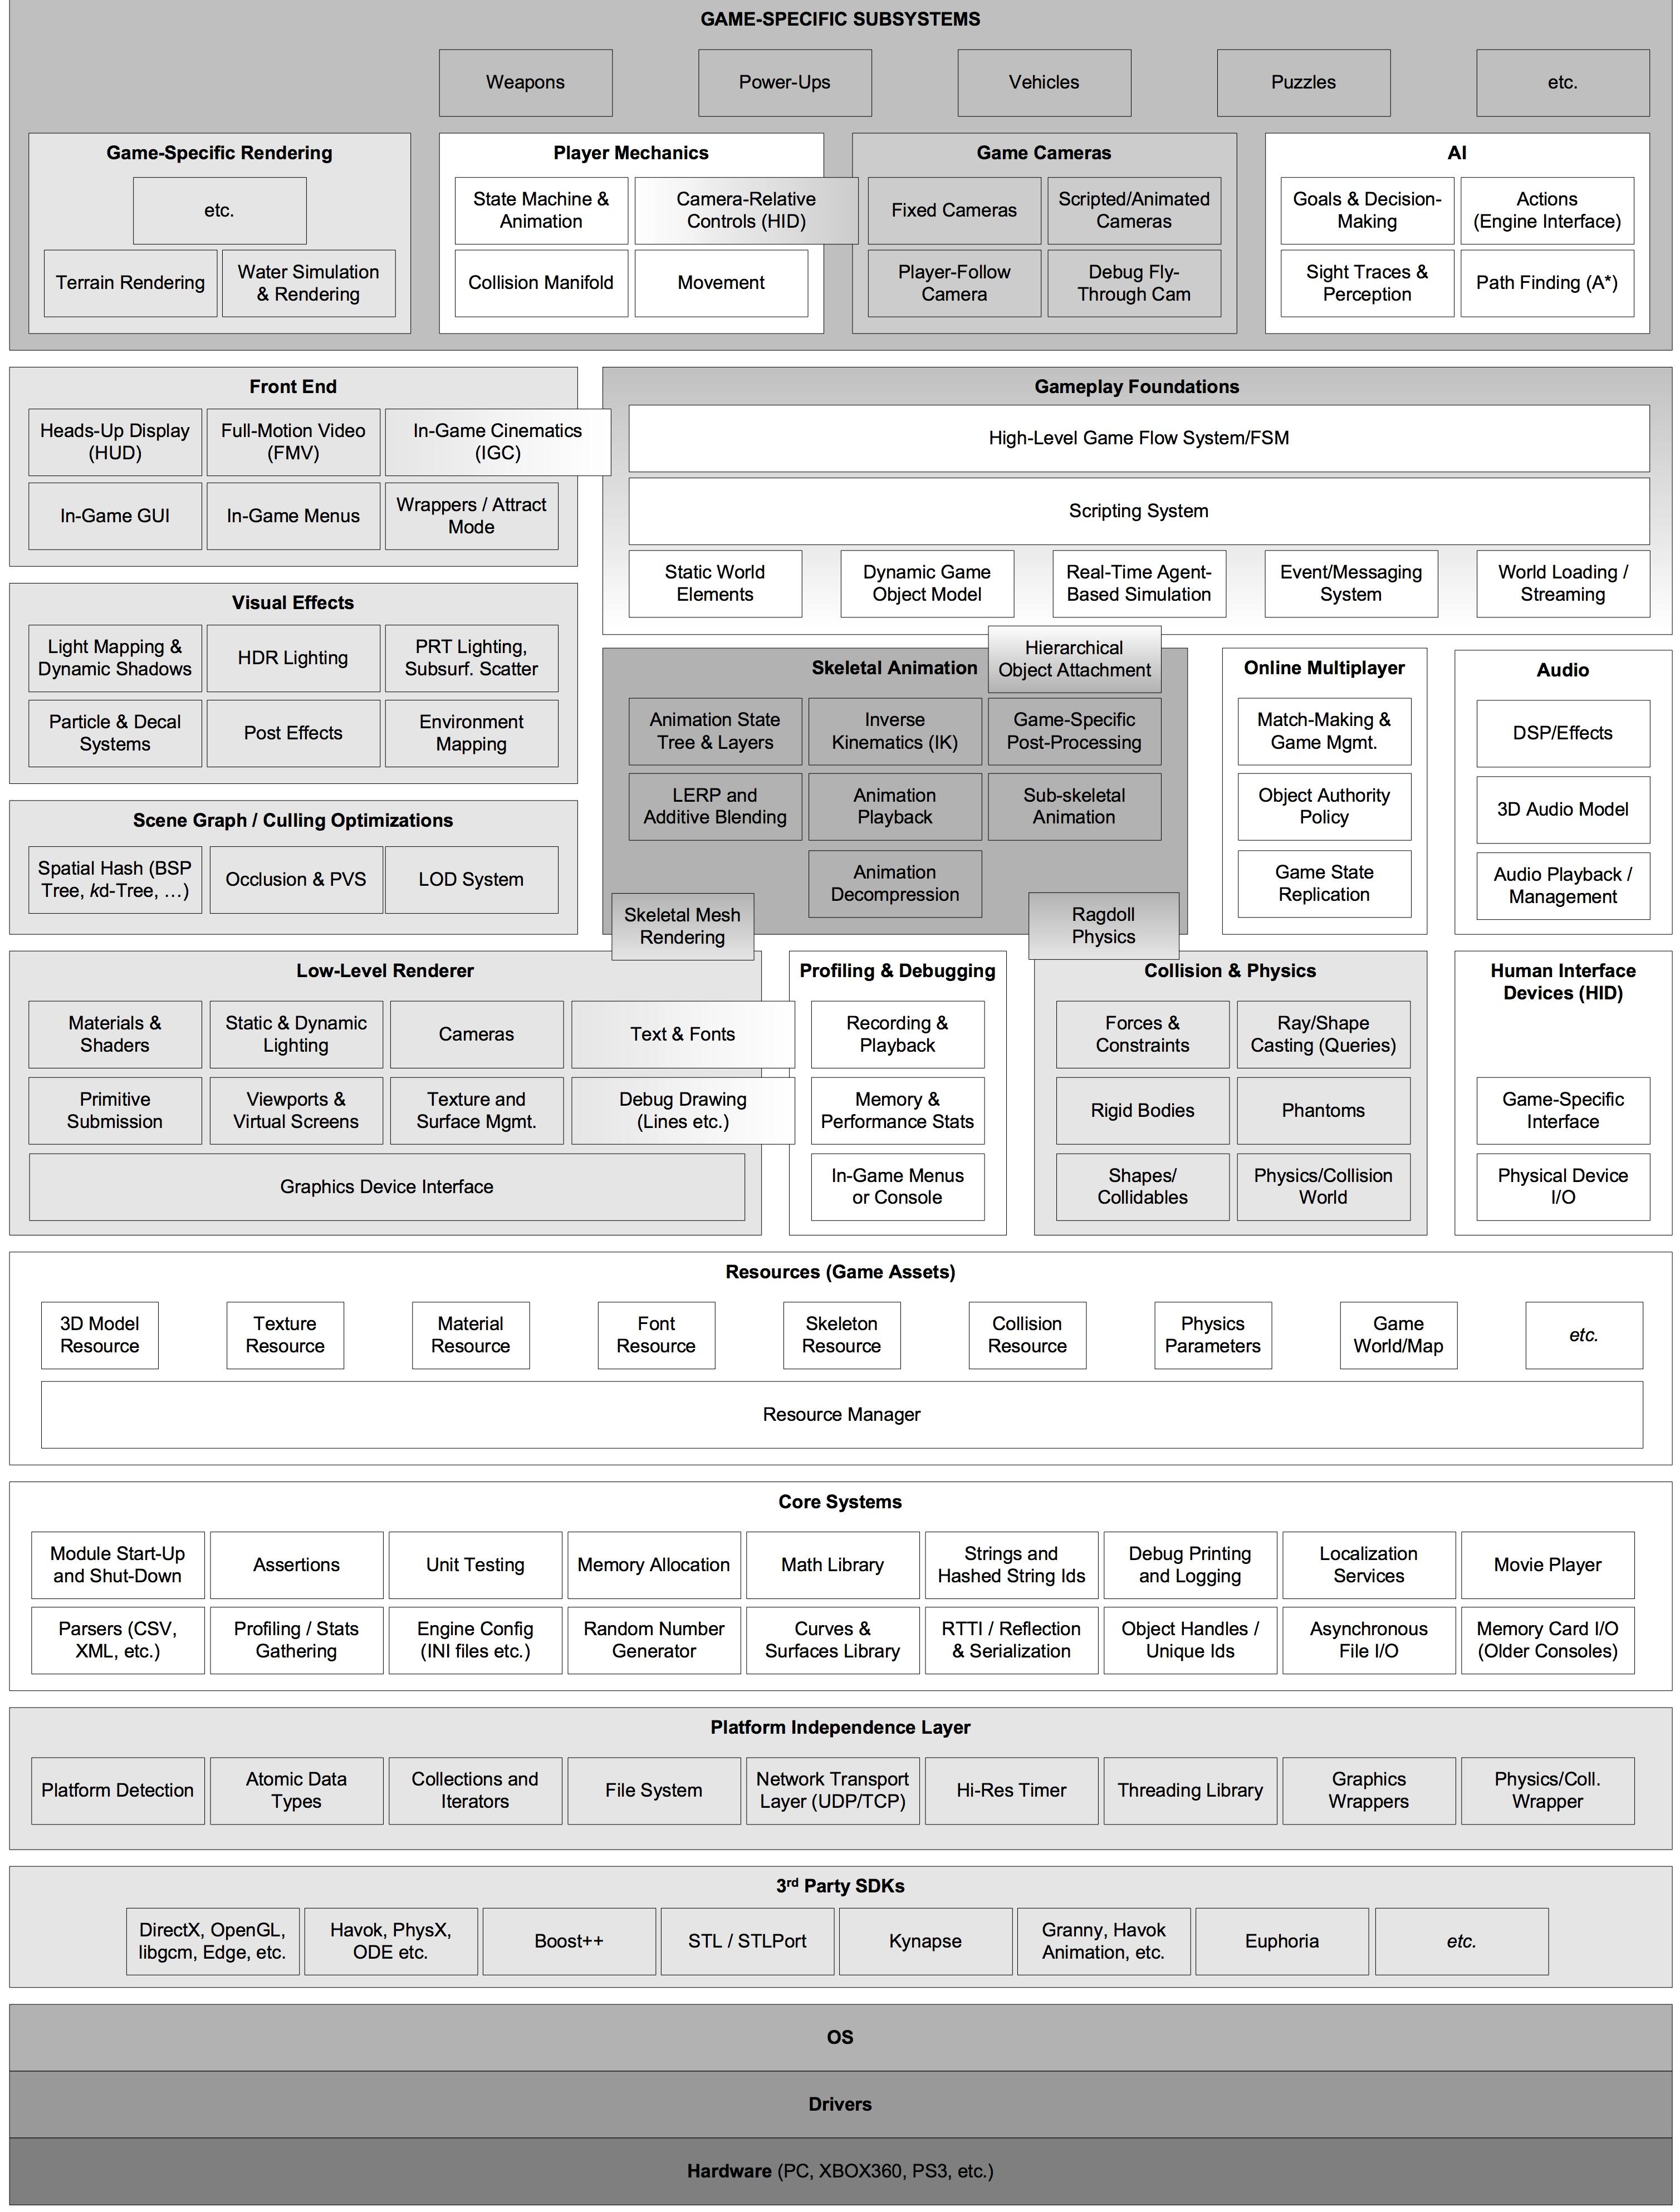
\includegraphics[width=\linewidth]{PICs/engine_runtime_arch.jpg}
	\caption{Illustration showing common modules grouped into distinct layers of a large scale engine solution}
	\label{fig:engine_runtime_arch}
\end{figure}

The complexity of modules in a layer grows when ascending through them from bottom to top. Where the lowermost layers include low-level systems essentially drivers \footnote{A program that controls or communicates with a hardware device}, platform-dependent 3\textsuperscript{rd} party \acp{SDK} or platform-independent abstraction components. Traversing the hierarchy upwards from core systems, over resource management, to general rendering and gameplay foundation modules, at one point the uppermost layers are reached. Those encompass game specific subsystems that can vary from one game to another. With the crude knowledge of the different layers involved in an engine it can be emphasized that a game engine is a highly complex software and building one is an endeavor that requires expertise, experience and time. It is important to properly reason out the architecture and uphold the focus onto the engine's goal. Maintaining focus while following the sketched out architecture will help to avoid unnecessary coupling and the implementation of irrelevant features or systems. 
The rest of this section will describe some modules from Figure \ref{fig:engine_runtime_arch} in-depth to investigate how they work and how they contribute to the combined whole.

\section{Memory Management}

One key constraint nearly every engine ha+s to fulfill is running games with a high frame rate. Because games are real-time simulations the time window for running gameplay logic and rendering a single frame is very limited. To complement this with discrete numbers for a game, running with 60 \ac{FPS} a slice of 16.6 ms can be used per single frame. To stay into this limits game developers came up with optimization techniques and algorithms that speed up calculations and processing. But the performance of code is not only dependent upon the efficiency of an applied algorithm but also how the program manages and uses its resources, especially memory. Controlling how an engine utilizes the \ac{RAM} is mandatory for guaranteeing high performance. The two most commonly applied memory usage optimizations are either reducing the amount of dynamic allocations at a game's runtime or allocating bigger sections of memory to store data in contiguous blocks. To solve these problems engines often implement custom memory allocators that have a better runtime performance then using the existing system allocator.

\subsection{Custom allocators}

Custom allocators are facilities that optimize dynamic memory allocations and reduce the performance penalty introduced by them. Its an allocator's main purpose to provide a source of memory the requester can work with. The process of finding a block of memory that fits the request is called an allocation. When requested memory is not needed anymore, the allocator takes it back and reuses it for another request if possible.
Almost all system programming languages come with a heap allocator, that can handle requests for memory at runtime. These so called \textit{heap allocations} are made by either calling \texttt{malloc() \& free()} (C) or \texttt{new \& delete operators} (C++). But caused by different aspects these allocations are rather slow. The performance penalty is mainly caused by two factors. At first, because any size of allocation has to be fulfilled by a heap allocator, it needs a lot of internal allocation management which introduces an overhead, making heap allocations costly. The second factor that contributes to the cost of dynamic allocations is that a context switch from user-mode to kernel-mode takes place before any allocation. 

To better understand why this introduces a performance penalty one has to know what divides the user- and kernel-mode. Many modern \acp{OS} distinguish between these two modes. A process, that is running in user-mode, often has no capabilities to directly talk with the underlying hardware, both for security and portability reasons. The way a user-mode process communicates with lower level systems is by issuing a \textit{system call}. Such calls trigger routines in the hardware that switches into the privileged kernel-mode, executing the requested kernel procedure while strictly controlling what is happening. After it terminates, the procedure forces a switch back into user-mode and the process continues at the point right after the system call.\cite{LinuxKernel}

And it is that context switching on system calls that slows down dynamic memory allocations. Whenever a call to \texttt{malloc()} or similar is issued, under the hood it forwards the request to a system call and the allocation is fulfilled in kernel-mode. But because every game engine needs some kind of dynamic allocations in some places, they have to be optimized. The common solution for this problem is a collection of customer allocators implemented in the engine's core systems. They resolve the problems bound to dynamic allocations by minimizing context switches and knowing the allocation patterns.
To reduce the overhead of system calls custom allocators satisfy allocation requests from a preallocated block of memory. This block can be acquired by the system's heap allocator (or with another approach that is described in the implementation section in chapter 6). After that block was allocated every further request for memory will stay in user-mode. Assuming the usage patterns of itself, a custom allocator can handle requests more efficiently than the general purpose heal allocator. Several different kinds of allocators are implemented and the user is responsible for knowing how the memory is used and which allocator fits the job best. That allows for reducing book keeping overhead and for better performing allocations.

The memory management module of a modern engine has a huge impact onto the general performance. It serves as the basis for many other modules and more high level ones, such as for example a container library, can be built on top of it. Being one of the modules that were implemented in the thesis' project, an even more in-depth insight into the internals of such a system and how it is implemented in Rust and C++ will be given in section \ref{mem_impl}. It will also describe how the different kinds of allocators work internally and how they can be easily combined with other utilities to form a versatile and well-performing system.

\section{Rendering}

One of the most complex parts of a game engine is the renderer. It encompasses many disciplines from graphics programming to algorithmic knowledge and there are many different architectures to choose from. This section will give a basic overview of how a renderer can be built but going into detail would quickly exceed the intention of this section. 
As many software solutions that become complex over time, a renderer is often separated into different layers. To recap them in a visually form, one can find them in Figure \ref{fig:engine_runtime_arch} under section \ref{engine_runtime_arch}. At the bottom of the architecture there is the low-level renderer. Its purpose is to render geometric primitives \footnote{Common primitives are points, lines or triangles} as quickly as possible without performing any redundant passes. To display the primitives onto a screen a renderer uses Graphics-\acp{SDK} such as OpenGL or DirectX. Cross-platform engines abstract the graphics \ac{API} used on a specific platform behind a layer called the \textit{graphics device interface}. This name is not a standard and can be any other one in the source code of different engines. It is the task of this interface to enumerate the available graphics devices and setup buffers \footnote{Memory blocks in the \ac{GPU} into which the renderer stores its generated values}.

\section{Job System}
\blindtext
\section{Gameplay systems}
\blindtext
\subsection{Entities}
\blindtext
\subsection{Scripting}
\blindtext
\section{Tools}
\blindtext
\subsection{Different approaches}
\blindtext
\subsection{Editor}
\blindtext
\subsection{Asset pipeline}
\blindtext